\chapter{Verification and Validation}
\label{chap:landice-vv}

% ===================================================
% ===================================================
%\section{Model Verification and Benchmarks}
% ===================================================
% ===================================================

MALI has been verified by a series of configurations that test different components of the code.
In some cases analytic solutions are used, but other tests rely on intercomparison with community benchmarks
that have been run previously by many different ice sheet models.

MALI currently includes 86 automated system regression tests that run the model for various
problems with analytic solutions or community benchmarks.
In addition to checking the accuracy of model answers,
some of the tests check that model restarts give bit-for-bit 
exact answers with longer runs without restart.
Some others check that the model gives bit-for-bit 
exact answers on different numbers of processors.
All but 20 of the longer running tests are run every time new features are added to the code,
and these tests each also include a check for answer changes.
The verification and benchmark descriptions below are the most 
important examples from the larger test suite.

\section{Halfar analytic solution}
In \citep{Halfar1981,Halfar1983}, Halfar
described an analytic solution for the time-evolving geometry of a radially-symmetric, isothermal dome of ice 
on a flat bed with no accumulation flowing under the shallow ice approximation.
This test provides an obvious test of the implementation of the shallow-ice velocity calculation and thickness evolution schemes
in numerical ice sheet models and a way to assess model order of convergence \citep{bueler2005,egholm2010}.
\citet{bueler2005} showed the Halfar test is the zero accumulation member of a family of analytic solutions,
but we apply the original Halfar test here.

In our application we use a dome following the analytic profile prescribed by \citet{Halfar1983} 
with an initial radius of 21213.2 m and an initial height of 707.1 m.
We run MALI with the shallow ice velocity solver and isothermal ice for 200 years
and then compare the modeled ice thickness to the analytic solution at 200 years.
We find the root mean square error in model thickness decreases as model grid spacing is decreased (Figure \ref{halfar}a).
The order of convergence of 0.78, consistent with the first-order approximation used for advection.

We also use this test to assess the accuracy of simulations with variable resolution.
We perform an addition run of the Halfar test using a variable resolution mesh
that has 1000 m cell spacing beyond a radius of 20 km that transitions to 
5000 m cell spacing at a radius of 3 km (Figure \ref{halfar}b),
generated with the JIGSAW(GEO) mesh generation tool \citep{Engwirda2017,Engwirda2017a}.
Root mean square error in thickness for this simulation is similar to 
that for the uniform 1000 m resolution case (Figure \ref{halfar}a),
providing confidence in the advection scheme applied to variable resolution meshes.
The variable resolution mesh has about half the cells of the 1000 m uniform resolution mesh.

\begin{figure}[t]
\includegraphics[width=7.3cm]{landice/figures/Halfar_convergence_and_mesh.pdf}
\caption{a) Root mean square error in ice thickness as a function of grid cell spacing for the Halfar dome after 200 years shown with black dots.  
The order of convergence is 0.78.
The red square show the RMS thickness error for the variable resolution mesh shown in b) with 1000 m spacing around the margin.
b) Mesh with resolution that varies linearly from 1000 m grid spacing beyond a radius of 20 km (thick white line) to 5000 m at a radius of 3 km (thin white line).  The ice thickness initial condition for the Halfar problem is shown.  This mesh requires 1265 cells for the 200 yr duration Halfar test case, while a uniform 1000 m resolution mesh requires 2323 cells.
}
\label{halfar}
\end{figure}

% \subsection{EISMINT-1}

% inception/evolution
%     EISMINT-1 - for SIA.  Compare to community benchmarks for inception/evolution
    
\section{EISMINT}
European Ice Sheet Modeling Initiative (EISMINT) model intercomparison
consisted of two phases designed to provide community benchmarks for shallow-ice models.
Both phases included experiments that grow a radially symmetric ice sheet on a flat bed to 
steady state with a prescribed surface mass balance.
The EISMINT intercomparisons test ice geometry evolution and ice temperature evolution with a variety of forcings.
\citet{bueler2007} describe an alternative tool for testing thermomechanical shallow-ice models
with artificially constructed exact solutions.
While their approach has the notable advantage of providing exact solutions,
we have not implemented the non-physical three-dimensional compensatory heat source
necessary for its implementation.
While we hope to use the verification of \citet{bueler2007} in the future,
for now we use the EISMINT intercomparison suites to test our implementation 
of thermal evolution and thermomechanical coupling.

The first phase \citep{huybrechts1996} (sometimes called EISMINT1) prescribes evolving ice geometry
and temperature, but the flow rate parameter $A$ is set to a prescribed value
so there is no thermomechanical coupling.
We have conducted the Moving Margin experiment with steady surface mass balance
and surface temperature forcing.
Following the specifications described by \citet{huybrechts1996},
we run the ice sheet to steady state over 200 ka.
We use the grid spacing prescribed by \citet{huybrechts1996} (50 km),
but due to the uniform Voronoi grid of hexagons we employ,
we have a slightly larger number of grid cells in our mesh (1080 vs 961).
At the end of the simulation, the modeled ice thickness at the center of the dome by MALI
is 2976.7 m, compared with a mean of 2978.0 $\pm$ 19.3 m for the ten three-dimensional models
reported by \citet{huybrechts1996}.
MALI achieves similar good agreement for basal homologous temperature at the center of the dome
with a value of $-13.09 ^{\circ}$ C, compared with $-13.34 \pm 0.56 ^{\circ}$ C for the six
models that reported temperature in \citet{huybrechts1996}.

The second phase of EISMINT \citep{payne2000} (sometimes called EISMINT2),
uses the basic configuration of the EISMINT1 Moving Margin experiment
but activates thermomechanical coupling through Eq. \ref{eq:mobalA}.
Two experiments (A and F) grow an ice sheet to steady state over 200 ka 
from an initial condition of no ice, but with different air temperature boundary conditions.
Additional experiments use the steady state solution from experiment A (the warmer air temperature case) as 
the initial condition to perturbations in the surface air temperature or surface mass balance forcings (experiments B, C, and D).
Because these experiments are thermomechanically coupled, they test
model ice dynamics and thickness and temperature evolution, as well as their coupling.
There is no analytic solution to these experiments,
but ten different models contributed results, yielding a range of behavior
against which to compare additional models.
Here we present MALI results for the five such experiments that prescribe no basal sliding (experiments A, B, C, D, F).
Our tests use the same grid spacing as prescribed by \citet{payne2000} (25 km),
again with a larger number of grid cells in our mesh (4464 vs 3721).

\citet{payne2000} report results for five basic glaciological quantities calculated by
ten different models, which we have summarized here with the corresponding values 
calculated by MALI (Table \ref{table-EISMINT2}).
All MALI results fall within the range of previously reported values,
except for volume change and divide thickness change in experiment C
and melt fraction change in experiment D.
However, these discrepancies are close to the range of results reported by \citet{payne2000},
and we consider temperature evolution and thermomechanical coupling within MALI
to be consistent with community models,
particularly given the difference in model grid and thickness evolution scheme.

A long-studied feature of the EISMINT2 intercomparison is the cold ``spokes'' that
appear in the basal temperature field of all models in Experiment F and, for some models, experiment A \citep{payne2000,Saito2006,bueler2007,brinkerhoff2013}.
MALI with shallow-ice velocity exhibits cold spokes for experiment F but not experiment A (Figure \ref{eismint-spokes}).
\citet{bueler2007} argue these spokes are a numerical instability that develops
when the derivative of the strain heating term is large.
\citet{brinkerhoff2013} demonstrate that the model VarGlaS avoids the formation of
these cold spokes. However, that model differs from previously analyzed models in several ways: 
it solves a three-dimensional, advective-diffusive description of an enthalpy formulation for energy conservation; it uses the Finite Element Method on unstructured meshes; conservation of momentum and energy are iterated on until they are consistent (rather than lagging energy and momentum solutions as in most other models). 
At present, it is unclear which combination of those features is responsible for preventing the formation of the cold spokes.

\begin{table*}[t]
\caption{EISMINT2 results for MALI shallow-ice model.
For each experiment, model name ``EISMINT2'' refers to mean and range of models reported in \citet{payne2000}, 
where we assume the range reported in by \citet{payne2000} is symmetric about the mean.
For experiments B, C, and D reported values are the change from experiment A results.
MALI results that lie outside the range of values in \citet{payne2000} are italicized.
}
\begin{tabular}{llccccc}
\tophline
Experiment & Model  &  Volume & Area & Melt fraction & Divide thickness & Divide basal temperature \\
           &        &  $10^6$ km$^3$ & $10^6$ km$^2$ & & m & K \\
\middlehline
A          & EISMINT2 & 2.128$\pm$0.0725 & 1.034$\pm$0.043 & 0.718$\pm$0.145 & 3688.3$\pm$48.3 & 255.6$\pm$1.4  \\
%          & MALI   & 2.095          & 1.024         & 0.635         & 3671.6        & 255.2  \\  % March 2016
           & MALI   & 2.097          & 1.030         & 0.637         & 3671.8        & 255.2  \\  % now
\middlehline
Experiment & Model  &  \% change & \% change & \% change & \% change & change (K)\\
\middlehline
B          & EISMINT2 & -2.589$\pm$0.4735 & 0.0$\pm$0.0 & 11.836$\pm$9.3345 & -4.9$\pm$0.658 & 4.6$\pm$0.259  \\
%          & MALI   & -2.310   & 0.0 & 18.000 & -5.013 & 4.6  \\  % March 2016
           & MALI   & -2.258   & 0.0 & 16.832 & -5.013 & 4.6  \\  % now
C          & EISMINT2 & -28.505$\pm$0.602 & -19.515$\pm$1.777 & -27.806$\pm$15.6855 & -12.9$\pm$0.7505 & 3.7$\pm$0.3075\\
%          & MALI   & \it{-27.469} & -19.672 & -34.170 & \it{-12.043} & 3.8  \\     % March 2016           
           & MALI   & \it{-27.529} & -20.179 & -35.521 & \it{-12.049} & 3.8  \\    % now
D          & EISMINT2 & -12.085$\pm$0.618 & -9.489$\pm$1.63 & -1.613$\pm$2.8725 & -2.2$\pm$0.266 & -0.2$\pm$0.03 \\
%           & MALI   & -12.301 & -9.519 & \it{-6.141} & -2.098 & -0.2  \\        % March 2016           
           & MALI   & -12.265 & -9.459 & \it{-5.216} & -2.092 & -0.2  \\        % now     
\bottomhline
\end{tabular}
\belowtable{} % Table Footnotes
 \label{table-EISMINT2}
\end{table*}


\begin{figure}[t]
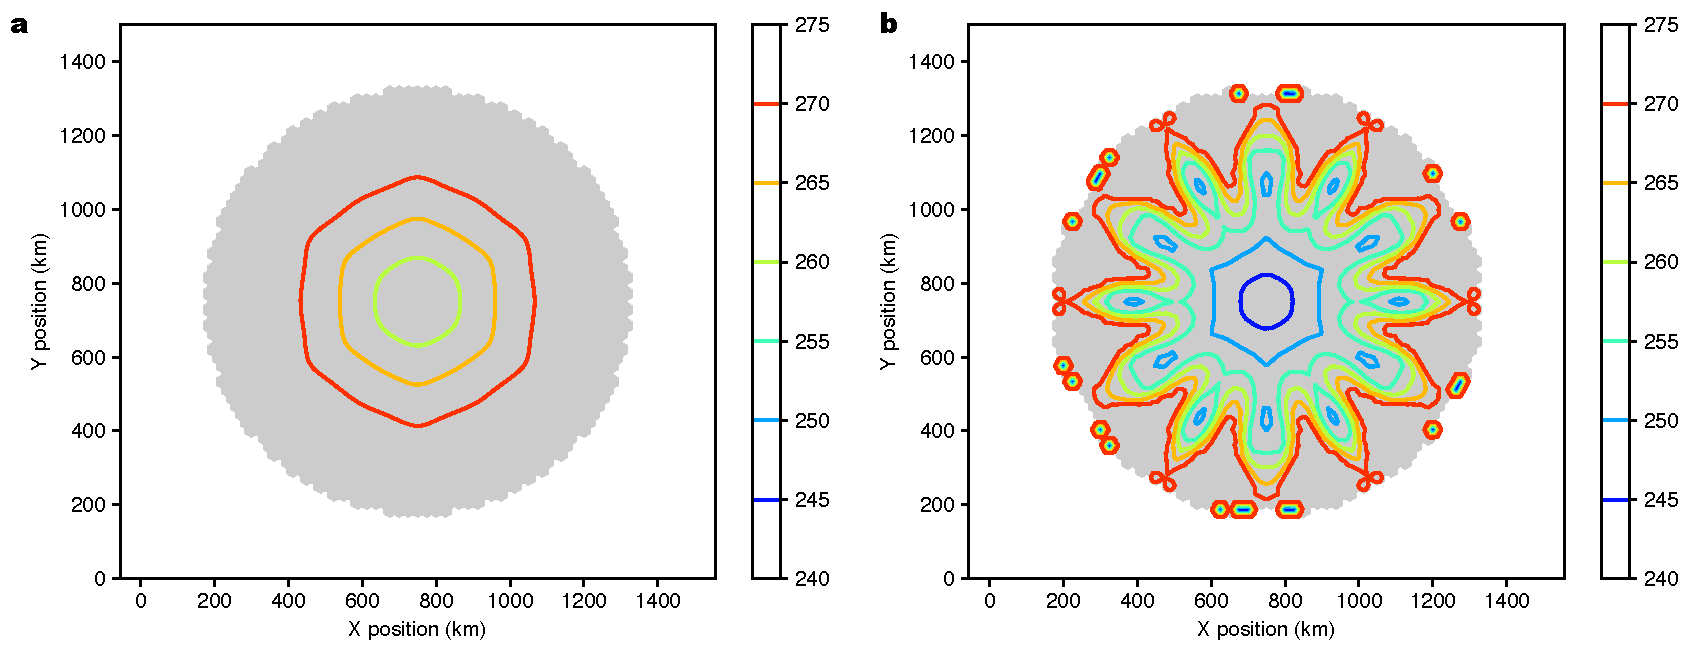
\includegraphics[width=16.0cm]{landice/figures/eismint_basal_temps.pdf}
\caption{a) Basal homologous temperature (K) for EISMINT2 Experiment A. b) Same for Experiment F.
Figures are plotted following \citet{payne2000}.
}
\label{eismint-spokes}
\end{figure}


\section{ISMIP-HOM}

The Ice Sheet Model Intercomparison Project-Higher Order Models (ISMIP-HOM)
is a set of community benchmark experiments for testing higher-order approximations of ice dynamics \citep{pattyn2008}.
\citet{tezaur2015a} describe results from the Albany-LI velocity solver for ISMIP-HOM 
experiments A (flow over a bumpy bed) and C (ice stream flow).
For all configurations of both tests, Albany-LI results were within one standard deviation of the mean
of first-order models presented in \citet{pattyn2008}, 
and showed excellent agreement with the similar first-order model formulation of \citet{perego2012}.
%\citet{tezaur2015a} also report excellent agreement with \citet{perego2012} (differences on the order of $10^{-10}$)
%for the confined shelf experiment described by Rommelaere...
These tests only require a single diagnostic solve of velocity,
and thus results through MALI match those of the standalone Albany-LI code it is using.

\section{MISMIP3d}

The Marine Ice Sheet Model Intercomparison Project-3d (MISMIP3d) is a community benchmark experiment
testing grounding line migration of marine ice sheets and includes nontrivial effects in all three dimensions \citep{pattyn2013}.
The experiments use a rectangular domain that is 800 km long in the longitudinal direction and 
50 km wide in the transverse direction, with the transverse direction making up half of a symmetric glacier.
The bedrock forms a sloping plane below sea level.
The first phase of the experiment (Stnd) is to build a steady state ice sheet
from a spatially uniform positive surface mass balance,
with a prescribed flow rate factor $A$ (no temperature calculation or coupling)
and prescribed basal friction for a nonlinear basal friction law.
A marine ice sheet forms with an unbuttressed floating ice shelf that terminates
at a fixed ice front at the edge of the domain.
From this steady state, the P75R perturbation experiment reduces basal friction by a maximum of 75\%
across a Gaussian ellipse centered where the Stnd grounding line position crosses the symmetry axis.
The perturbation is applied for 100 years, resulting in a curved grounding line that is advanced along the symmetry axis.
After the completion of P75S, a reversibility experiment named P75R removes the basal friction perturbation
and allows the ice sheet to relax back towards the Stnd state.

\citet{pattyn2013} report results from 33 models of varying complexity and applied at resolution ranging from 0.1 to 20 km.
Participating models used depth-integrated shallow-shelf or L1L1/L2L2 approximations, hybrid shallow-ice/shallow-shelf approximation, or the complete Stokes equations; there were no three-dimensional first-order approximation models included.
This relatively simple experiment revealed a number of key features necessary to accurately model even a simple marine ice sheet.
Insufficient grid resolution prevented reversibility of the steady state grounding line position after experiments P75S and P75R.
Reversibility required grid resolution well below 1 km without a subgrid parameterization of grounding line position,
and grids a couple times coarser with a grounding line parameterization \citep{pattyn2013,Gladstone2010a}.
The steady state grounding line position in the Stnd experiment was dependent on the stress approximation employed, 
with Stokes model calculating grounding lines the farthest upstream and models that simplify or eliminate vertical shearing 
(e.g., shallow shelf) having grounding lines farther downstream, by up to 100 km.
With these features resolved, numerical error due to grounding line motion is smaller than errors due to parameter uncertainty \citep{pattyn2013}.

We find MALI using the Albany-LI first-order velocity solver is able to resolve the MISMIP3d experiments
satisfactorily compared to the \citet{pattyn2013} benchmark results
when using a grid resolution of 500 m with grounding line parameterization.  
Results at 1 km resolution with grounding line parameterization are close to fully resolved.
We first assess grid convergence by comparing the position of the steady state grounding line in the Stnd experiment
for a range of resolutions against our highest resolution configuration of 250 m (Figure \ref{mismip-convergence}).
Without a grounding line parameterization, the grounding line position appears unconverged,
but with the grounding line parameterization, grid convergence occurs at 500 m resolution.
The converged grounding line position for the Stnd experiment with MALI is 534 km.
This represents the first results published for a three-dimensional, first-order stress approximation
that we are aware of, and this grounding line position falls between that of the L1L2 and Stokes models reported
by \citet{pattyn2013}, consistent with the intermediate level of approximation of our model.
The dissertation work by \citet{Leguy2015a} reported similar results for the Blatter-Pattyn velocity solver with grounding line parameterization in the Community Ice Sheet Model.

Reversibility of the P75S and P75R experiments shows the same grid resolution requirement 
of 500 m,
while the 1 km simulation with grounding line parameterization is close to reversible
(Figure \ref{mismip-p75}).
Our highest resolution 250 m simulation without grounding line parameterization
does show reversibility at the end of P75R (not shown), but the results differ somewhat
from the runs with grounding line parameterization due to the differing starting position
determined from the Stnd experiment.
Thus for marine ice sheets with similar configuration to the MISMIP3d test,
we recommend using MALI with the grounding line parameterization and a resolution of 1 km or less.

The transient results using the MALI three-dimensional first-order stress balance
look most similar to those of the ``SCO6'' L1L2 model presented by \citet{pattyn2013}
in that it takes about 50 years for the grounding line to reach its most advanced position
during P75S.
In contrast, the Stokes models took notably longer and the models with reduced or missing representation of membrane stresses reached their furthest advance within the first couple decades \citep{pattyn2013}.

In addition to MISMIP3d, we have used MALI to perform the MISMIP+ experiments \citep{Asay-Davis2016}.  
These results are included in the MISMIP+ results paper in preparation and not shown here.


\begin{figure}[t]
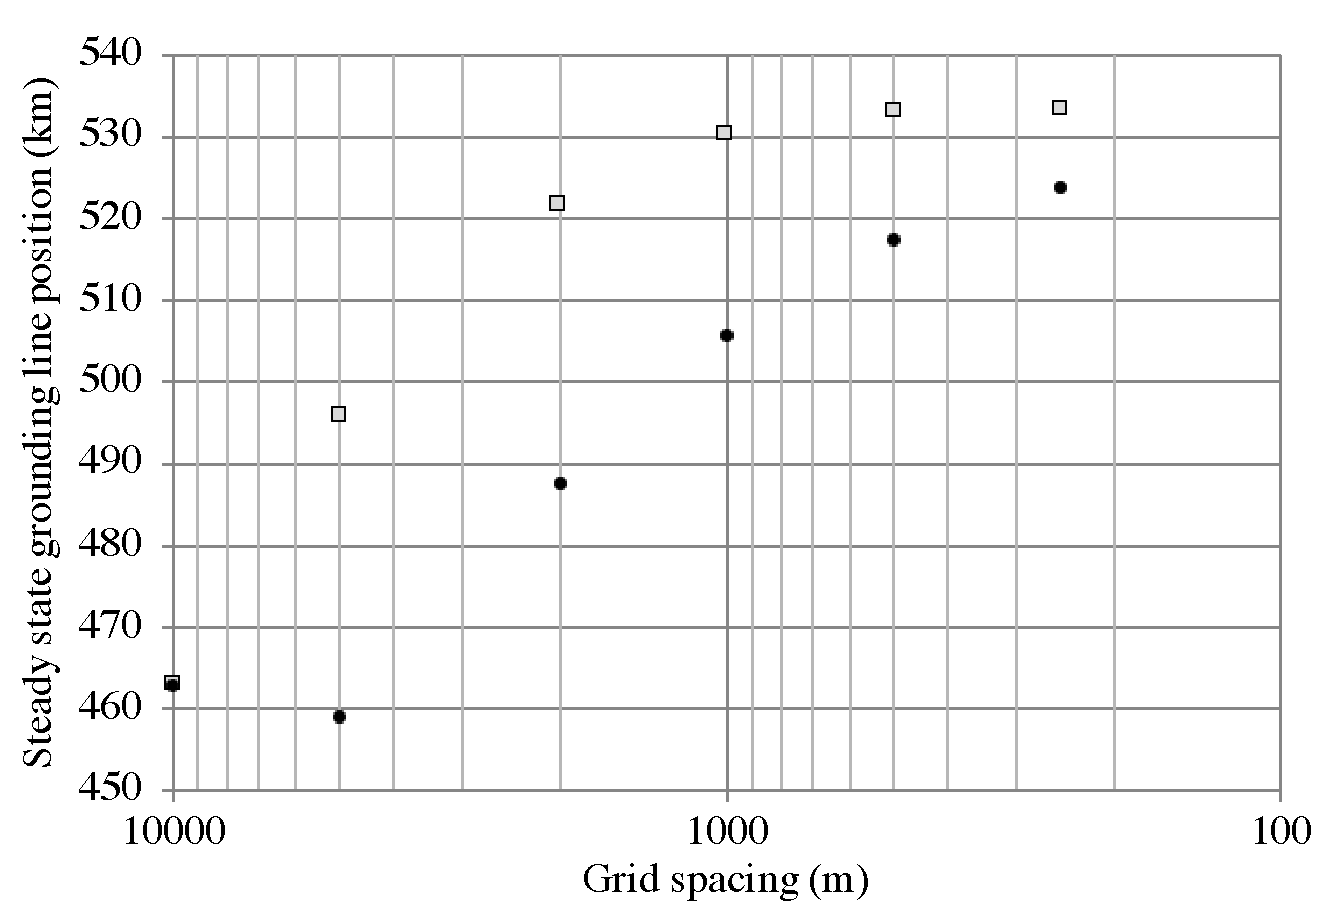
\includegraphics[width=10.0cm]{landice/figures/MISMIP3d_Stnd_convergence_plot.pdf}
\caption{
Grid resolution convergence for MISMIP3d Stnd experiment with (gray squares) and without (black circles) grounding line parameterization.
}
\label{mismip-convergence}
\end{figure}

\begin{figure}[t]
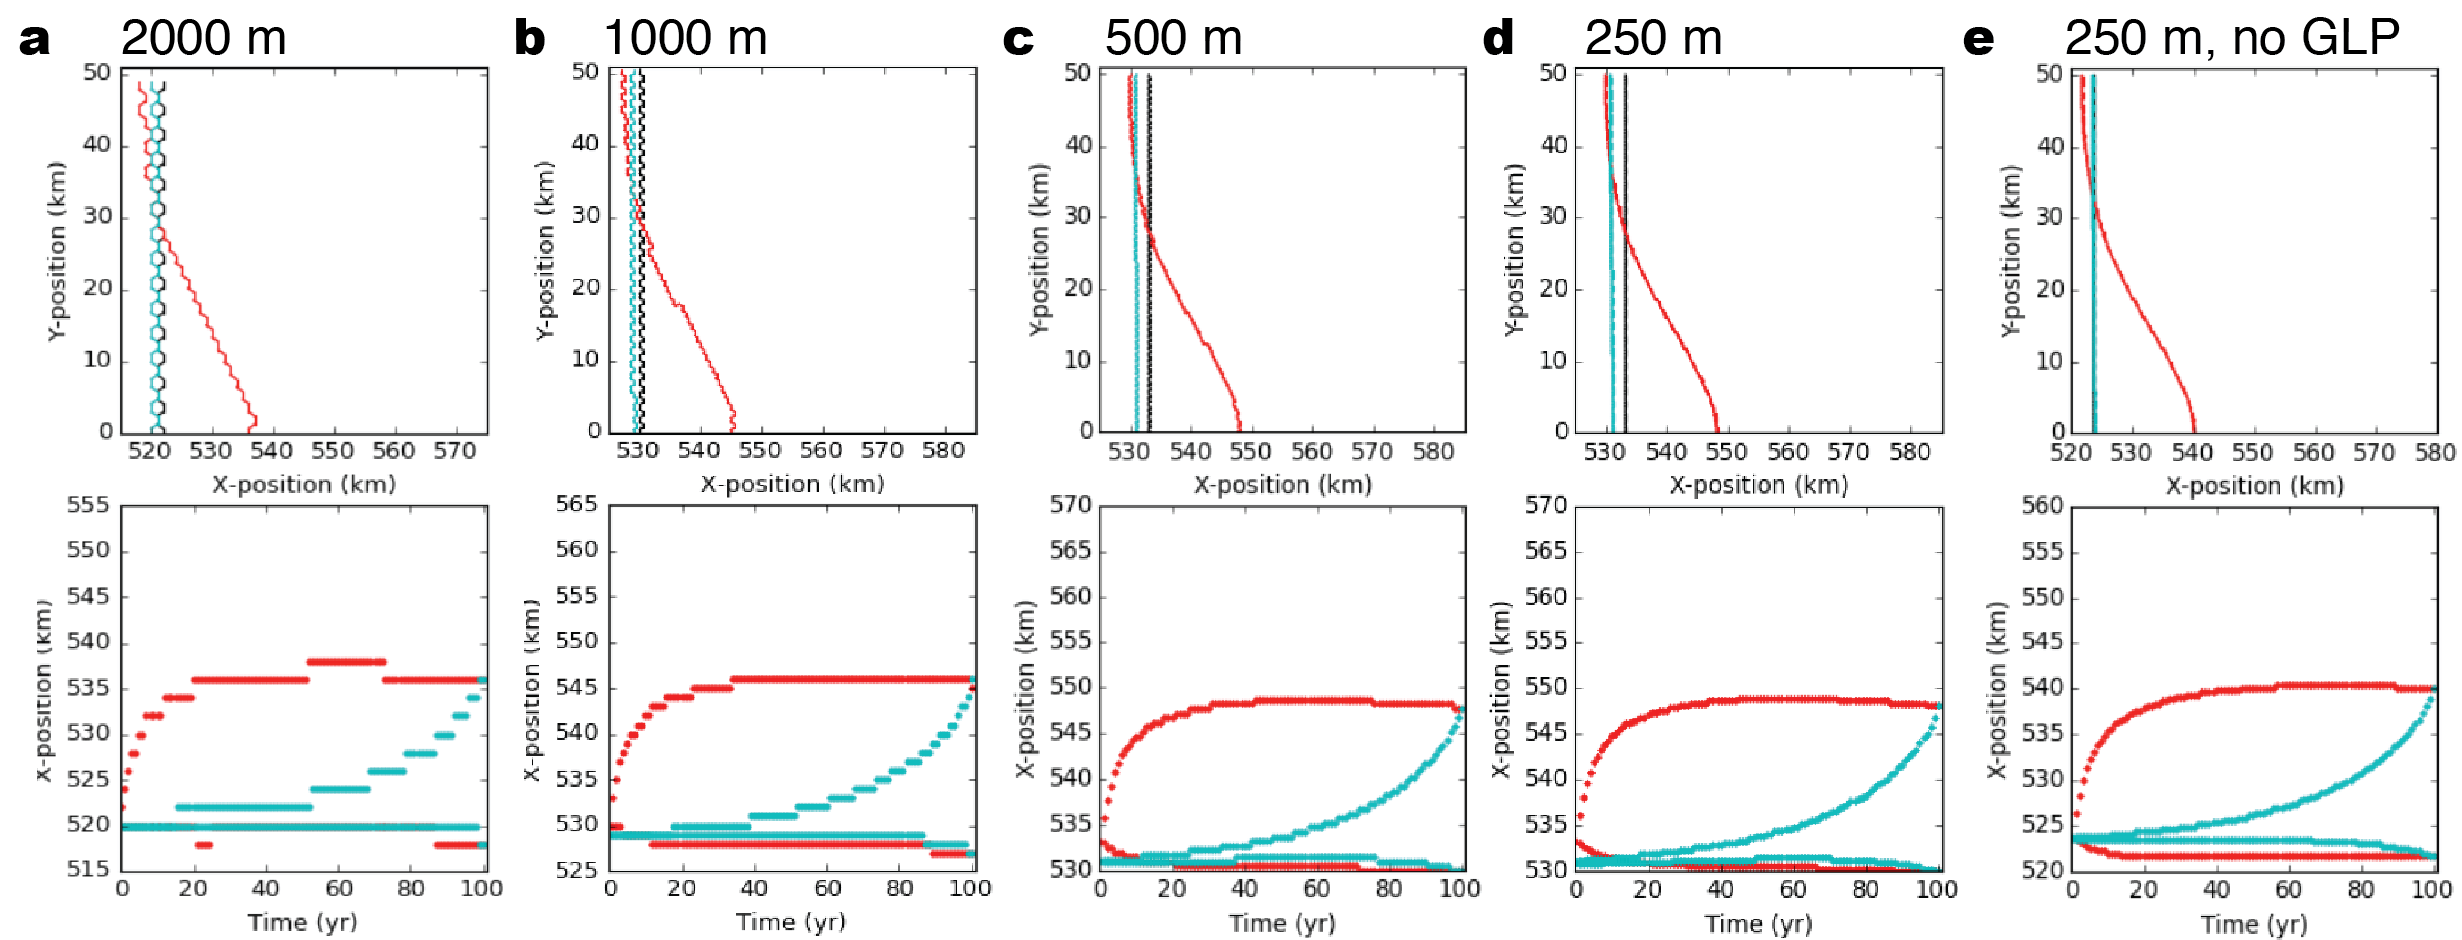
\includegraphics[width=16.0cm]{landice/figures/mismip3d.png}
\caption{
Results of the MISMIP3d P75R and P75S experiments from MALI at increasing grid resolution:
a) 2000 m, b) 1000 m, c) 500 m, d) 250 m.
Results for 250 m without grounding line parameterization (e) are also shown for reference.
Plots follow conventions of Figures 5 and 6 in \citet{pattyn2013}.
Upper plot in each subplot shows steady state grounding line positions for steady-state spin-up (black), P75S (red), and P75R (blue) experiments.
Lower plot in each subplot shows grounding line position with time for P75R (red) and P75S (blue) at y=0 km (top curves) and y=50 km (bottom curves).
500 m and 250 m results are nearly identical.  
250 m results without grounding line parameterization are intermediate of those at 1000 m and 2000 m resolution with grounding line parameterization.
}
\label{mismip-p75}
\end{figure}
